%% For double-blind review submission, w/o CCS and ACM Reference (max submission space)
\documentclass[sigplan,10pt,review,anonymous]{acmart}
\settopmatter{printfolios=true,printccs=false,printacmref=false}
%% For double-blind review submission, w/ CCS and ACM Reference
%\documentclass[sigplan,review,anonymous]{acmart}\settopmatter{printfolios=true}
%% For single-blind review submission, w/o CCS and ACM Reference (max submission space)
%\documentclass[sigplan,review]{acmart}\settopmatter{printfolios=true,printccs=false,printacmref=false}
%% For single-blind review submission, w/ CCS and ACM Reference
%\documentclass[sigplan,review]{acmart}\settopmatter{printfolios=true}
%% For final camera-ready submission, w/ required CCS and ACM Reference
%\documentclass[sigplan]{acmart}\settopmatter{}


%% Conference information
%% Supplied to authors by publisher for camera-ready submission;
%% use defaults for review submission.
\acmConference[PL'18]{ACM SIGPLAN Conference on Programming Languages}{January 01--03, 2018}{New York, NY, USA}
\acmYear{2018}
\acmISBN{} % \acmISBN{978-x-xxxx-xxxx-x/YY/MM}
\acmDOI{} % \acmDOI{10.1145/nnnnnnn.nnnnnnn}
\startPage{1}

%% Copyright information
%% Supplied to authors (based on authors' rights management selection;
%% see authors.acm.org) by publisher for camera-ready submission;
%% use 'none' for review submission.
\setcopyright{none}
%\setcopyright{acmcopyright}
%\setcopyright{acmlicensed}
%\setcopyright{rightsretained}
%\copyrightyear{2018}           %% If different from \acmYear

%% Bibliography style
\bibliographystyle{ACM-Reference-Format}
%% Citation style
%\citestyle{acmauthoryear}  %% For author/year citations
%\citestyle{acmnumeric}     %% For numeric citations
%\setcitestyle{nosort}      %% With 'acmnumeric', to disable automatic
                            %% sorting of references within a single citation;
                            %% e.g., \cite{Smith99,Carpenter05,Baker12}
                            %% rendered as [14,5,2] rather than [2,5,14].
%\setcitesyle{nocompress}   %% With 'acmnumeric', to disable automatic
                            %% compression of sequential references within a
                            %% single citation;
                            %% e.g., \cite{Baker12,Baker14,Baker16}
                            %% rendered as [2,3,4] rather than [2-4].


%%%%%%%%%%%%%%%%%%%%%%%%%%%%%%%%%%%%%%%%%%%%%%%%%%%%%%%%%%%%%%%%%%%%%%
%% Note: Authors migrating a paper from traditional SIGPLAN
%% proceedings format to PACMPL format must update the
%% '\documentclass' and topmatter commands above; see
%% 'acmart-pacmpl-template.tex'.
%%%%%%%%%%%%%%%%%%%%%%%%%%%%%%%%%%%%%%%%%%%%%%%%%%%%%%%%%%%%%%%%%%%%%%


%% Some recommended packages.
\usepackage{booktabs}   %% For formal tables:
                        %% http://ctan.org/pkg/booktabs
% \usepackage{subcaption} %% For complex figures with subfigures/subcaptions
                        %% http://ctan.org/pkg/subcaption

%usepackage[disable]{todonotes} % add the "disable" package option when ready to submit
\usepackage{todonotes} % add the "disable" package option when ready to submit, see above line.
\usepackage{alltt}
\usepackage{mathptmx}
\usepackage{courier}
\usepackage[scaled]{helvet} % see www.ctan.org/get/macros/latex/required/psnfss/psnfss2e.pdf
\DeclareMathAlphabet{\mathsf}{OT1}{phv}{m}{n}
\usepackage{siunitx}
\usepackage{listings}
\usepackage{multirow}
\usepackage{subfig}
\usepackage{cancel}
\usepackage{xspace}
\usepackage[inline]{enumitem}
\usepackage{relsize}

%
% todo
%
\DeclareRobustCommand{\steve}[1]{\todo[fancyline,color=green!40,size=\scriptsize]{\textsf{S: #1}}\xspace}
\DeclareRobustCommand{\kathryn}[1]{\todo[fancyline,color=red!20,size=\scriptsize]{\textsf{K:#1}}\xspace}

% switch these around so the no-op ones are used before submitting
\newcommand{\pending}[1]{\textcolor{red}{#1\xspace}}
\newcommand{\checked}[1]{\textcolor{green}{#1\xspace}}
%\newcommand{\pending}[1]{#1\xspace}
%\newcommand{\checked}[1]{#1\xspace}

%
% benchmarks
%
\newcommand*{\textbm}[1]{\textsf{#1}}

\newcommand{\specjvm}{\textbm{SPECjvm}\xspace}
\newcommand{\jess}{\textbm{jess}\xspace}
\newcommand{\raytrace}{\textbm{raytrace}\xspace}
\newcommand{\db}{\textbm{db}\xspace}
\newcommand{\javac}{\textbm{javac}\xspace}
\newcommand{\jack}{\textbm{jack}\xspace}
\newcommand{\compress}{\textbm{compress}\xspace}
\newcommand{\mpegaudio}{\textbm{mpegaudio}\xspace}
\newcommand{\mtrt}{\textbm{mtrt}\xspace}
\newcommand{\jbb}{\textbm{jbb2000}\xspace}
\newcommand{\specjbb}{\textbm{SPECjbb2000}\xspace}
\newcommand{\newspecjbb}{\textbm{SPECjbb2005}\xspace}
\newcommand{\psjbb}{\textbm{pseudojbb}\xspace}
\newcommand{\pjbb}{\textbm{pjbb2005}\xspace}
\newcommand{\dacapo}{\textbm{DaCapo}\xspace}
\newcommand{\dacapover}{\textbm{DaCapo v.06-10-MR2}\xspace}
\newcommand{\antlr}{\textbm{antlr}\xspace}
\newcommand{\bloat}{\textbm{bloat}\xspace}
\newcommand{\eclipse}{\textbm{eclipse}\xspace}
\newcommand{\fop}{\textbm{fop}\xspace}
\newcommand{\hsqldb}{\textbm{hsqldb}\xspace}
\newcommand{\jython}{\textbm{jython}\xspace}
\newcommand{\pmd}{\textbm{pmd}\xspace}
\newcommand{\xalan}{\textbm{xalan}\xspace}
\newcommand{\chart}{\textbm{chart}\xspace}
\newcommand{\luindex}{\textbm{luindex}\xspace}
\newcommand{\lusearch}{\textbm{lusearch}\xspace}
\newcommand{\lusearchfix}{\textbm{lusearch-fix}\xspace}
\newcommand{\avrora}{\textbm{avrora}\xspace}
\newcommand{\sunflow}{\textbm{sunflow}\xspace}

%
% Stuff for pretty printing the source code using listings.sty
%

\lstloadlanguages{java}
\lstset{
  numbers=left,
  numberstyle=\tiny\sffamily,
  stepnumber=1,
  numbersep=1em,
  language=java,                         % the language
  basicstyle=\scriptsize\ttfamily,     % the basic font family to use
  commentstyle=\scriptsize\it\ttfamily,% the font for comments
  stringstyle=\ttfamily,
  escapechar={\$},
  morekeywords={Address, Word, Offset, Extent, ObjectReference}
}

% This command allows us to conviniently put java text inline.
\DeclareRobustCommand{\textjava}[1]{{\lstset{basicstyle=\footnotesize\ttfamily}\lstinline@#1@}}


\begin{document}

%% Title information
\title[Short Title]{Full Title}         %% [Short Title] is optional;
                                        %% when present, will be used in
                                        %% header instead of Full Title.
\titlenote{with title note}             %% \titlenote is optional;
                                        %% can be repeated if necessary;
                                        %% contents suppressed with 'anonymous'
\subtitle{Subtitle}                     %% \subtitle is optional
\subtitlenote{with subtitle note}       %% \subtitlenote is optional;
                                        %% can be repeated if necessary;
                                        %% contents suppressed with 'anonymous'


%% Author information
%% Contents and number of authors suppressed with 'anonymous'.
%% Each author should be introduced by \author, followed by
%% \authornote (optional), \orcid (optional), \affiliation, and
%% \email.
%% An author may have multiple affiliations and/or emails; repeat the
%% appropriate command.
%% Many elements are not rendered, but should be provided for metadata
%% extraction tools.

%% Author with single affiliation.
\author{First1 Last1}
\authornote{with author1 note}          %% \authornote is optional;
                                        %% can be repeated if necessary
\orcid{nnnn-nnnn-nnnn-nnnn}             %% \orcid is optional
\affiliation{
  \position{Position1}
  \department{Department1}              %% \department is recommended
  \institution{Institution1}            %% \institution is required
  \streetaddress{Street1 Address1}
  \city{City1}
  \state{State1}
  \postcode{Post-Code1}
  \country{Country1}                    %% \country is recommended
}
\email{first1.last1@inst1.edu}          %% \email is recommended

%% Author with two affiliations and emails.
\author{First2 Last2}
\authornote{with author2 note}          %% \authornote is optional;
                                        %% can be repeated if necessary
\orcid{nnnn-nnnn-nnnn-nnnn}             %% \orcid is optional
\affiliation{
  \position{Position2a}
  \department{Department2a}             %% \department is recommended
  \institution{Institution2a}           %% \institution is required
  \streetaddress{Street2a Address2a}
  \city{City2a}
  \state{State2a}
  \postcode{Post-Code2a}
  \country{Country2a}                   %% \country is recommended
}
\email{first2.last2@inst2a.com}         %% \email is recommended
\affiliation{
  \position{Position2b}
  \department{Department2b}             %% \department is recommended
  \institution{Institution2b}           %% \institution is required
  \streetaddress{Street3b Address2b}
  \city{City2b}
  \state{State2b}
  \postcode{Post-Code2b}
  \country{Country2b}                   %% \country is recommended
}
\email{first2.last2@inst2b.org}         %% \email is recommended


%% Abstract
%% Note: \begin{abstract}...\end{abstract} environment must come
%% before \maketitle command
\begin{abstract}
%
% problem
% contribution
% result
% meaning
%
  A good abstract and introduction should clearly state what problem
  the paper is addressing (e.g., making GC go faster, improving the
  user experience when programs have bugs, finding bugs), the
  contribution toward solving this problem (e.g., a GC that combines
  locality and efficiency, a new mechanism for finding leaks, a new
  programming language), the results (e.g., programs run faster or do
  not crash or are easier to understand), and include a summary
  statement that indicates what this means (e.g., GC can be a
  performance win instead of a cost, we can build better performing
  VMs now, we can keep programs running with errors of type y, or
  programmers can write programs more succinctly).
\end{abstract}

%%% Local Variables:
%%% mode: latex
%%% TeX-master: "paper"
%%% End:



%% 2012 ACM Computing Classification System (CSS) concepts
%% Generate at 'http://dl.acm.org/ccs/ccs.cfm'.
\begin{CCSXML}
<ccs2012>
<concept>
<concept_id>10011007.10011006.10011008</concept_id>
<concept_desc>Software and its engineering~General programming languages</concept_desc>
<concept_significance>500</concept_significance>
</concept>
<concept>
<concept_id>10003456.10003457.10003521.10003525</concept_id>
<concept_desc>Social and professional topics~History of programming languages</concept_desc>
<concept_significance>300</concept_significance>
</concept>
</ccs2012>
\end{CCSXML}

\ccsdesc[500]{Software and its engineering~General programming languages}
\ccsdesc[300]{Social and professional topics~History of programming languages}
%% End of generated code


%% Keywords
%% comma separated list
\keywords{keyword1, keyword2, keyword3}  %% \keywords are mandatory in final camera-ready submission


%% \maketitle
%% Note: \maketitle command must come after title commands, author
%% commands, abstract environment, Computing Classification System
%% environment and commands, and keywords command.
\maketitle


\section{Introduction}

Structure the introduction along the same lines as the abstract.
Expand on the problem, contribution, result, and meaning in one or two
paragraphs on each.

% problem

% contribution

% result

% meaning

A few grammatical notes.  Elminate passive voice.  Passivity
introduces ambiguity (Who is the actor?).  Ambiguity is occasionally a
useful device, but as a rule it is the antithesis of effective
scientific communication, so should be avoided.  Do not use a citation
as a noun, always use it as a footnote.  For example, instead of
``\cite{BH:04} measure barrier overheads.''  say ``\citeauthor{BH:04}
measure barrier overheads~\cite{BH:04}.''  Do not use an unqualified
``this'' as the noun of your sentence. For example, instead of ``This
makes caches rock.''  say ``This locality of reference makes caches
rock.''

Some other points of style.  When writing numbers with units, you
should insert a small space (\textjava{\\,}) between the number and
the units.  For example, use `\textjava{2.8\\,GHz}', which renders as
2.8\,GHz.  The space is there for correctness (see NIST standards on
units), and the small space both typesets it nicely and ensures the
unit does not wrap onto a different line from the number.

The \textjava{todonotes} package provides nice
\todo[fancyline,color=green,size=\footnotesize]{This is a test of
  todonotes} tricks for adding todo items (\textjava{\\todo}) and
notes to your draft document.  You can make macros with \kathryn{This
  is a note from Kathryn.} color-coded notes from each of the authors.
When you are ready to submit, you should silence them all with the
\textjava{disable} package option.  Figure~\ref{fig:todo}
shows\steve{Here's one from Steve.}  the package's
\textjava{\\missingfigure} macro, which is a nice way to make
place-holders.

When there are numbers for checking before submit, you can use \pending{12456}
to highlight the number. After you check the number, switch it to
\checked{12456}. When you submit the paper, change the these two macros to submit
version, then the color will disappear.

\begin{figure}
  \centering
  \missingfigure{There's a figure missing here}
  \caption{An example of a missing figure, using \textjava{todonotes}'
    \textjava{\\missingfigure} macro.}
  \label{fig:todo}
\end{figure}

There are good tools for automating the process of running latex.  I
discourage you from using a Makefile.  If your editor does not do the
job for you, you should probably use \textjava{latexmk}, which is
bundled as part of the standard texlive distribution.  There is an
example configuration file provided in this directory.  Copy it into
your home director with the name \textjava{.latexmkrc} (notice the
dot).

Gratuitous citation to generate a few bib entries \cite{BH:04,SBF:12,YBFH:12}.

%%% Local Variables:
%%% mode: latex
%%% TeX-master: "paper"
%%% End:


\section{Related Work}
\label{sec:related}

Putting related work at the front of the paper (after the intro) in
all submissions.  Your reviewers (PC members) are busy, must often
read 20 or more papers, and are not necessarily expert on your topic.
If you succinctly explain the limitations of previous work and how
your work \emph{relates} to all the prior work and hopefully improves
over it, the PC member will be more motivated to recommend accepting
your submission.

It may make sense to move related work toward the end of the paper for
a camera-ready version (which is, after all, for a different
audience).


%%% Local Variables:
%%% mode: latex
%%% TeX-master: "paper.tex"
%%% End:


\section{Analysis}
\label{sec:analysis}



\begin{figure}
  \centering
  \subfloat[Read\label{fig:codea}]{\lstinputlisting{code/read.java}}\\
  \subfloat[Write\label{fig:codeb}]{\lstinputlisting{code/write.java}}
  \caption{An example of including source code, and using subfigures.}
  \label{fig:code}
\end{figure}

Figure~\ref{fig:code} shows how to use the \textjava{listings} package
to include source code in the document.  It also shows how to use
\textjava{subfig} to generate subfloats.  You can reference a subfloat
just like a float.  For example,
Figure~\ref{fig:code}\subref{fig:codea} is an example of a read
barrier.

%%% Local Variables:
%%% mode: latex
%%% TeX-master: "paper"
%%% End:


\section{Methodology}
\label{sec:methodology}

%%% Local Variables: 
%%% mode: latex
%%% TeX-master: "paper"
%%% End: 


\section{Results}
\label{sec:results}

\begin{figure}
  \centering
  \subfloat[Increments\label{fig:incnew}]{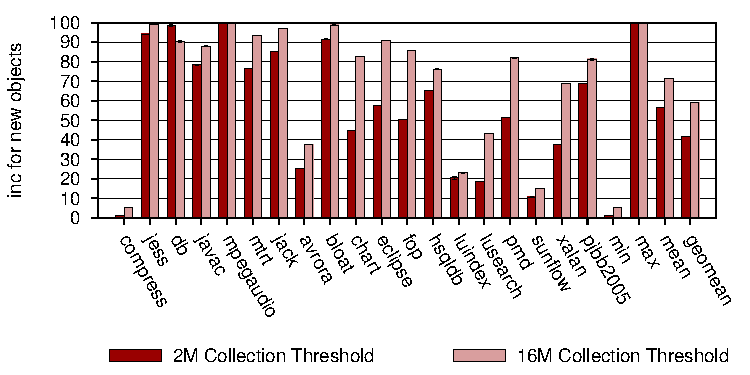
\includegraphics[width=\columnwidth]{figs/incnew}}\\
  \subfloat[Decrements\label{fig:decnew}]{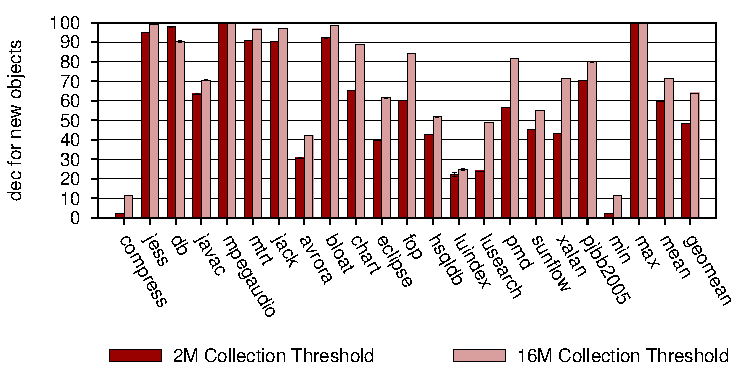
\includegraphics[width=\columnwidth]{figs/decnew}}
  \caption{New objects are responsible for the majority of reference
    counting operations.  We show here the fraction of (a) increments
    and (b) decrements that are due to objects allocated within the
    most recent 2\,MB and 16\,MB of objects allocated.}
  \label{fig:incdecnew}
\end{figure}

Figure~\ref{fig:incdecnew} is an example of a figure with subfloats
and an example of a reasonable caption.  Notice how the caption is
somewhat self-contained.  The reader could glance at this figure and
understand something of it without being required to dig into the
text. The graphs in Figure~\ref{fig:incdecnew} are too small --- only
just acceptable.

This is an example of using the \textsf{\textbackslash siunitx}
package: The job took \SI{321}{\micro\second}, with an average current
of \SI{3.24}{\ampere}, totalling \SI{1.13}{\milli\watt}.  These macros
ensure correct typsetting --- note the small space between number and
units and the non-italicized mu for the \si{\micro\second}.  The
package provides very powerfull options for formatting tables (not yet
used in the example given in this template!).  Check out the package
documentation.

\begin{table*}
  \newcommand{\timemetric}{$\Delta\mathsf{t}$}
  \newcommand{\instmetric}{$\Delta\mathsf{i}$}
  \newcommand{\imissmetric}{$\Delta\mathsf{i_{miss}}$}
  \newcommand{\cpimetric}{$\mathsmaller{\Delta\mathsf{t}/\Delta\mathsf{i}}$\xspace}
  \centering
   {  \relsize{-1}   % use relsize to scale the entire table uniformly.
  \input table/bigexample.tex
  }
  \caption{Overheads (\%) in time, instructions, and i-cache misses for the
    primitive barriers on the i7.  The the first six column groups summarize
    the performance for each barrier, showing percentage increase in
    execution time (\timemetric), retired instructions (\instmetric), and
    instruction cache misses (\imissmetric) compared to the base case where
    no barriers are used.  The right-most two column groups give results for
    the compound barriers.  The figures in grey beneath the corresponding
    arithmetic mean report 95\% confidence intervals.}
    \label{tab:big}
\end{table*}

Table~\ref{tab:big} is a pretty good example of a large table.  It's
probably the largest table we've ever published in a regular
conference paper.  Don't do it lightly.  A table like this should be
generated with a script or at least with the assistance of an emacs
macro.  There is a massive amount of information in this table, and
without very careful typesetting, it would be a disaster and
unreadable.
\\

\noindent
Notice:
\begin{enumerate}
\item that the font is sans serif,
\item that there are no vertical lines,
\item that differences in whitespace between the columns and breaks in
  the horizontal lines serve to group the data into clusters,
\item how the secondary (but nonetheless important) data about
  confidence intervals is typset in a very small font in grey,
\item how benchmark suites are separately aggregated and expressed in
  bold,
\item how both means and geomeans are provided, and
\item how mins and maxs across all the benchmarks are at the bottom.
\end{enumerate}

%%% Local Variables:
%%% mode: latex
%%% TeX-master: "paper"
%%% End:


\section{Conclusion}

The conclusion should mirror the abstract, in a retrospective voice.
There should be greater emphasis on `meaning' (i.e. the fourth element
of the abstract structure, which speaks to the significance and
consequences of this work).

%%% Local Variables: 
%%% mode: latex
%%% TeX-master: "paper"
%%% End: 


\ \\ 
Kathryn's conflict list:

\begin{itemize}
\item All UT faculty and students
\item All Microsoft Research
\item Mathew Arnold, IBM
\item Steve Blackburn, ANU
\item Keith Cooper, Rice
\item Perry Cheng, IBM
\item Amer Diwan, Google
\item Mike Hicks, UMD
\item Martin Hirzel, IBM
\item Tony Hosking, Purdue
\item Robert Grimm, NYU
\item David Grove, IBM
\item Sam Guyer, Tufts
\item Eliot Moss, UMass
\item Nick Nethercote, Mozilla
\item Darko Stefanovic, UNM
\item Zhenlin Wang, MTU

\end{itemize}

\ \\ 
Steve's conflict list:

\begin{itemize}
\item All ANU
\item Mathew Arnold, IBM
\item Perry Cheng, IBM
\item Amer Diwan, Google
\item Daniel Frampton, Microsoft
\item Matthias Hauswirth, U. Lugano
\item Martin Hirzel, IBM
\item Tony Hosking, Purdue
\item David Grove, IBM
\item Kathryn McKinley, Microsoft Research
\item Eliot Moss, UMass
\item Jenn Sartor, U. Gent
\item Peter Sweeney, IBM

\end{itemize}

%%% Local Variables: 
%%% mode: latex
%%% TeX-master: "paper"
%%% End: 


Cross refs are a nice way to keep the bibliography style consistent
and clean, and also allows the drop-in replacement of different
citation styles for conferences.  However, if you use this, you
probably want to pass the option \textjava{-min-crossrefs=2000} to
\textjava{bibtex} to avoid it generating entries for each of the
crossreferenced fields (the default value is \textjava{2}, which means
an entry for the venue will be generated if there are two or more
citations that use that crossref).  If you use \textjava{latexmk} or
any other such tool for running latex, you should set this option in
your config file.  The \textjava{latexmkrc} file provided with this
example does that.

%% Acknowledgments
\begin{acks}                            %% acks environment is optional
                                        %% contents suppressed with 'anonymous'
  %% Commands \grantsponsor{<sponsorID>}{<name>}{<url>} and
  %% \grantnum[<url>]{<sponsorID>}{<number>} should be used to
  %% acknowledge financial support and will be used by metadata
  %% extraction tools.
  This material is based upon work supported by the
  \grantsponsor{GS100000001}{National Science
    Foundation}{http://dx.doi.org/10.13039/100000001} under Grant
  No.~\grantnum{GS100000001}{nnnnnnn} and Grant
  No.~\grantnum{GS100000001}{mmmmmmm}.  Any opinions, findings, and
  conclusions or recommendations expressed in this material are those
  of the author and do not necessarily reflect the views of the
  National Science Foundation.
\end{acks}


%% Bibliography
\bibliography{paper}


%% Appendix
\appendix
\section{Appendix}

Text of appendix \ldots

\end{document}
